% Created 2024-01-17 Wed 09:56
% Intended LaTeX compiler: pdflatex
\documentclass[bigger]{beamer}
\usepackage[utf8]{inputenc}
\usepackage[T1]{fontenc}
\usepackage{graphicx}
\usepackage{longtable}
\usepackage{wrapfig}
\usepackage{rotating}
\usepackage[normalem]{ulem}
\usepackage{amsmath}
\usepackage{amssymb}
\usepackage{capt-of}
\usepackage{hyperref}
\usepackage[spanish, mexico]{babel}
\uselanguage{Spanish}
\languagepath{Spanish}
\usepackage{mathtools}
%%%%%%%%%%%%%%%%%%%%%%%%%%%%%%%%%%%%%%%%%%%%%%%%%%%%%%%%%%%%%%%%%%%%%%%%%%%%%%%%%%%%%%%%
%% TEX code to draw an external link symbol                                           %%
%% See https://tex.stackexchange.com/questions/99316/symbol-for-external-links/294990 %%
%%%%%%%%%%%%%%%%%%%%%%%%%%%%%%%%%%%%%%%%%%%%%%%%%%%%%%%%%%%%%%%%%%%%%%%%%%%%%%%%%%%%%%%%

\usepackage{tikz}

\newcommand{\ExternalLink}{%
    \tikz[x=1.2ex, y=1.2ex, baseline=-0.05ex]{% 
        \begin{scope}[x=1ex, y=1ex]
            \clip (-0.1,-0.1) 
                --++ (-0, 1.2) 
                --++ (0.6, 0) 
                --++ (0, -0.6) 
                --++ (0.6, 0) 
                --++ (0, -1);
            \path[draw, 
                line width = 0.5, 
                rounded corners=0.5] 
                (0,0) rectangle (1,1);
        \end{scope}
        \path[draw, line width = 0.5] (0.5, 0.5) 
            -- (1, 1);
        \path[draw, line width = 0.5] (0.6, 1) 
            -- (1, 1) -- (1, 0.6);
    }
}


\usepackage{fixpauseincludegraphics}
\usetheme[height=20pt]{Rochester}
\usecolortheme{wolverine}
\author{Schwartz y Riker}
\date{17-1-2024}
\title{La teoría de la elección social}
\setbeamertemplate{footline}[frame number]{}
\setbeamertemplate{navigation symbols}{}
\expandafter\def\expandafter\insertshorttitle\expandafter{%
\insertshorttitle\hfill%
\insertframenumber}
%  \insertframenumber\,/\,\inserttotalframenumber}

















\hypersetup{
 pdfauthor={Schwartz y Riker},
 pdftitle={La teoría de la elección social},
 pdfkeywords={},
 pdfsubject={},
 pdfcreator={Emacs 27.1 (Org mode 9.6.12)}, 
 pdflang={Spanish}}
\begin{document}

\maketitle
\begin{frame}{Outline}
\tableofcontents
\end{frame}

\setbeamercovered{transparent}

\section{Qué es, qué busca}
\label{sec:orgcf908aa}
\begin{frame}[label={sec:orgd0f06d8}]{\emph{Social Choice Theory}}
\begin{columns}
\begin{column}{0.45\columnwidth}
Ni las instituciones democráticas, ni sus mecanismos son perfectos
\end{column}
\begin{column}{0.55\columnwidth}
\footnotesize
\emph{Democracy is the worst form of government, except for all those other forms that have been tried from time to time} --- Churchill
\pause \bigskip \bigskip
\end{column}
\end{columns}
\begin{itemize}[<+->]
\item XVIII descubrió paradojas que mantienen ocupados a teólogos, filósofos, matemáticos, economistas, politólogos
\item XX: excepto una, no hay regla inmune a resultados anómalos y consecuencias inesperadas, todas son manipulables
\item La excepción es\ldots{} la dictadura
\end{itemize}
\bigskip \pause
\begin{block}{En la agenda}
Disectaremos los engranes de la democracia en busca de las \alert{propiedades de sus mecanismos}
\end{block}
\end{frame}

\begin{frame}[label={sec:org0f77309}]{El voto: condición necesaria de la democracia}
\emph{Social choice} es una teoría de agregación de preferencias

\pause \bigskip

\begin{columns}
\begin{column}{0.45\columnwidth}
Desde la Antigüedad, las democracias deciden mediante \uline{votaciones}

\bigskip

\(\rightarrow\) estudio del \alert{mecanismo}: su potencial, sus límites
\end{column}

\begin{column}{0.55\columnwidth}
\centering
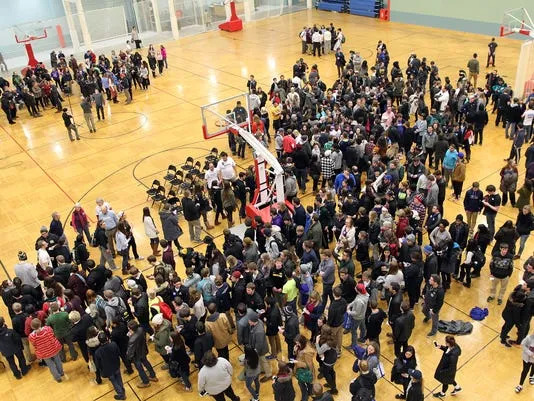
\includegraphics[width=.85\textwidth]{./pics/iowa-2016-caucus.jpg} \\[0pt]
\href{https://www.youtube.com/watch?v=tCvMtkEVqdA}{\footnotesize{\ExternalLink Caucus Iowa clásica}}
\end{column}
\end{columns}
\end{frame}


\begin{frame}[label={sec:org87638dc}]{El voto: condición necesaria de la democracia}
Obviedad: en una decisión colegiada, lo correcto y justo es elegir por mayoría de votos

\bigskip

Tan obvio, razonable y universalmente aceptado, que nadie cuestionó el axioma básico de la elección por escrutinio: 

que \alert{la mayoría de votos expresa la voluntad del electorado}

\pause \bigskip

\bigskip \pause
\begin{block}{Lento arribo}
\begin{itemize}
\item 1781: Borda fue el primero en cuestionar la validez del axioma
\end{itemize}
\pause
\begin{itemize}
\item Común percibir al mecanismo como algo \alert{anodino}, autoevidente: mero recuento de los votos
\item La Rev. Francesa descubrió que no es nada trivial, pero el interés no llegó hasta el XX
\end{itemize}
\end{block}
\end{frame}
\begin{frame}[label={sec:orgcf63f7d}]{Jean-Charles de Borda}
\begin{center}
\begin{tabular}{lll}
\uline{Lupe} 8 votos (electa) & \uline{Max} 7 votos & \uline{Ana} 6 votos\\[0pt]
\end{tabular}
\end{center}

\pause

\begin{block}{Los ordenamientos son fundamentales}
No se atiende preferencias entre los que quedan fuera. 
\begin{center}
\begin{tabular}{llllll}
8 votantes & Lupe & \(>_i\) & Ana & \(>_i\) & Max\\[0pt]
7 votantes & Max & \(>_i\) & Ana & \(>_i\) & Lupe\\[0pt]
6 votantes & Ana & \(>_i\) & Max & \(>_i\) & Lupe\\[0pt]
\end{tabular}
\end{center}
\end{block}

\bigskip \pause
\begin{itemize}
\item Enfrentados por pares:
\end{itemize}
\begin{center}
\begin{tabular}{lll}
Max > Lupe & Ana > Lupe & Ana > Max\\[0pt]
\end{tabular}
\end{center}
\begin{itemize}
\item Gana Ana y Lupe fuera\ldots{} resultado exacto opuesto
\item También propuso un método preferencial
\end{itemize}
\end{frame}
\begin{frame}[label={sec:org186a94c}]{El voto: condición necesaria de la democracia}
\begin{block}{Votación:}
\centering
transforma \alert{preferencias individuales} en una \alert{decisión colectiva}
\end{block}

\bigskip \pause
La \emph{teoría de la elección social} nos enseñará que
\begin{itemize}
\item ni las preferencias por sí solas determinan el voto
\item ni el voto por sí solo determina la decisión final
\end{itemize}

\bigskip \pause
\(\rightarrow\) potencial y límites del \alert{mecanismo} democrático
\end{frame}

\section{La regla de mayoría}
\label{sec:org65166af}

\begin{frame}[label={sec:orgb2369ae}]{La regla de mayoría}
\begin{description}
\item[{Sentido amplio}] forma de gobierno donde la mayoría se impone (p.ej. sistema \emph{Westminster})
\item[{Sentido estricto}] regla de votación para decidir entre dos alternativas
\end{description}
\bigskip \pause
\setbeamercolor{myblockcolor}{bg=cyan,fg=white}
\begin{beamercolorbox}{myblockcolor}
\begin{itemize}
\item La elección presidencial de 2024 no será por regla de mayoría ¿por cuál?
\item La CPEUM usa una nomenclatura distinta ¿cuál?
\end{itemize}
\end{beamercolorbox}
\end{frame}

\begin{frame}[label={sec:org0af03b8}]{CPEUM}
\begin{block}{Mayoría}
\begin{itemize}
\item simple = \emph{plurality}
\item absoluta \(\approx\) \emph{majority}
\item calificada = \emph{supermajority}
\end{itemize}
\end{block}
\end{frame}


\begin{frame}[label={sec:org6270a92}]{Ubicuidad de la regla}
Natural usar la de mayoría cuando un grupo debe optar entre dos alternativas (y pluralidad con > 2)

\bigskip
Tiene ventajas prácticas:
\begin{itemize}
\item todos iguales
\item mismas oportunidades para las alternativas
\item fácilmente decisiva
\end{itemize}
\bigskip
\begin{block}{\(\rightarrow\) Percepción muy generalizada:}
Es una regla \alert{justa} -- ventajas también son normativas
\end{block}
\end{frame}

\begin{frame}[label={sec:orgac81cb3}]{Ciclicidad}
\centering
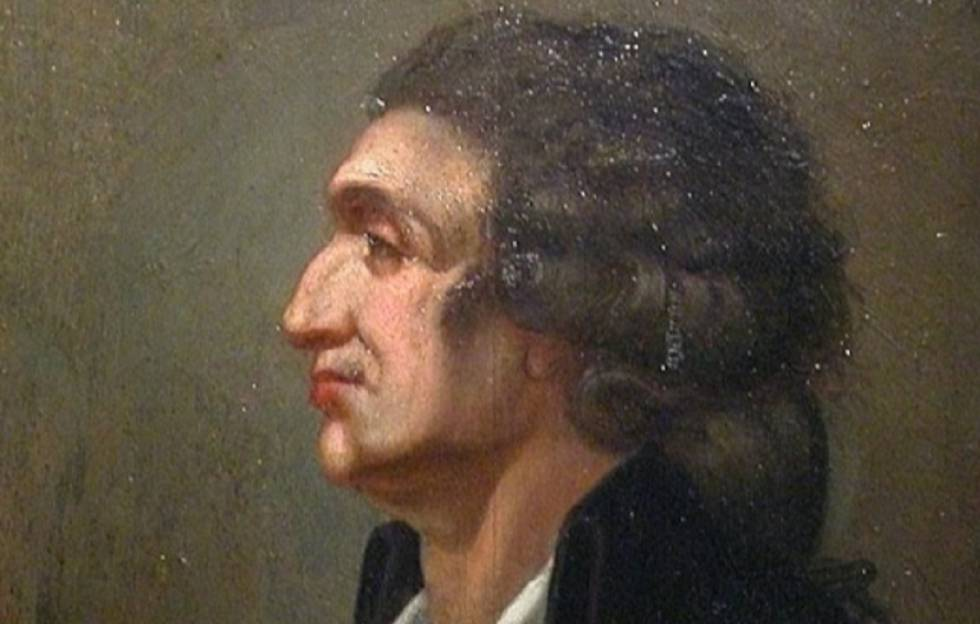
\includegraphics[width=.4\textwidth]{./pics/condorcet.jpg} 

Marquis de Condorcet (1743--94) \\[0pt]
La conjunción de individuos coherentes puede ser incoherente
\bigskip
\begin{itemize}
\item En elección con 3+ alternativas (candidatos, mociones)
\item al compararlas por pares
\item es posible que \alert{ninguna} resulte victoriosa
\end{itemize}
\end{frame}
\begin{frame}[label={sec:orgc79e8a5}]{Fines y medios de la democracia}
\centering
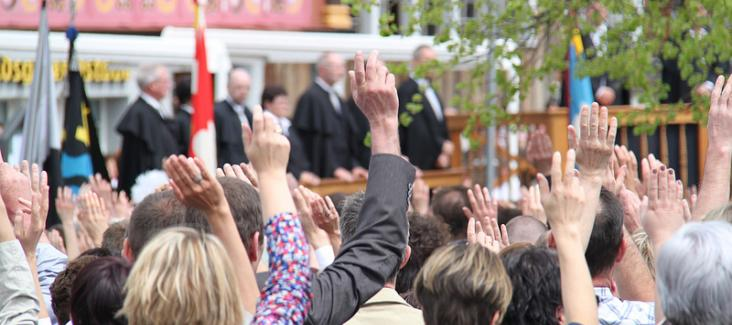
\includegraphics[width=.6\textwidth]{./pics/2014-02-10_swiss_people_vote.jpg} 
\bigskip
\begin{itemize}
\item fin: construir el entorno humano en comunidad
\end{itemize}

\begin{itemize}
\item medio: participativa y colectivamente  \(\rightarrow\) \alert{votando}
\end{itemize}
\bigskip \pause
Pregunta: ¿el medio es capaz de realizar el fin? \\[0pt]
\bigskip
Parece evidente, \\[0pt]
pero la paradoja de Condorcet recorre como fantasma
\end{frame}
\begin{frame}[label={sec:org756b4b6}]{Mayorías intransitivas}
\begin{center}
\begin{tabular}{lll}
\(V_1\) & \(V_2\) & \(V_3\)\\[0pt]
\hline
\(x\) Morena & \(y\) PAN & \(z\) PRI\\[0pt]
\(y\) PAN & \(z\) PRI & \(x\) Morena\\[0pt]
\(z\) PRI & \(x\) Morena & \(y\) PAN\\[0pt]
\end{tabular}
\end{center}
\bigskip \pause
\(\text{PAN} < \text{Morena} \;\;\; \text{Morena} < \text{PRI} \;\;\; \text{PRI} < \text{PAN}\)
\(\rightarrow \text{ciclo}\) 
\end{frame}
\begin{frame}[label={sec:org2e8aa43}]{Elección primaria 2020}
\centering
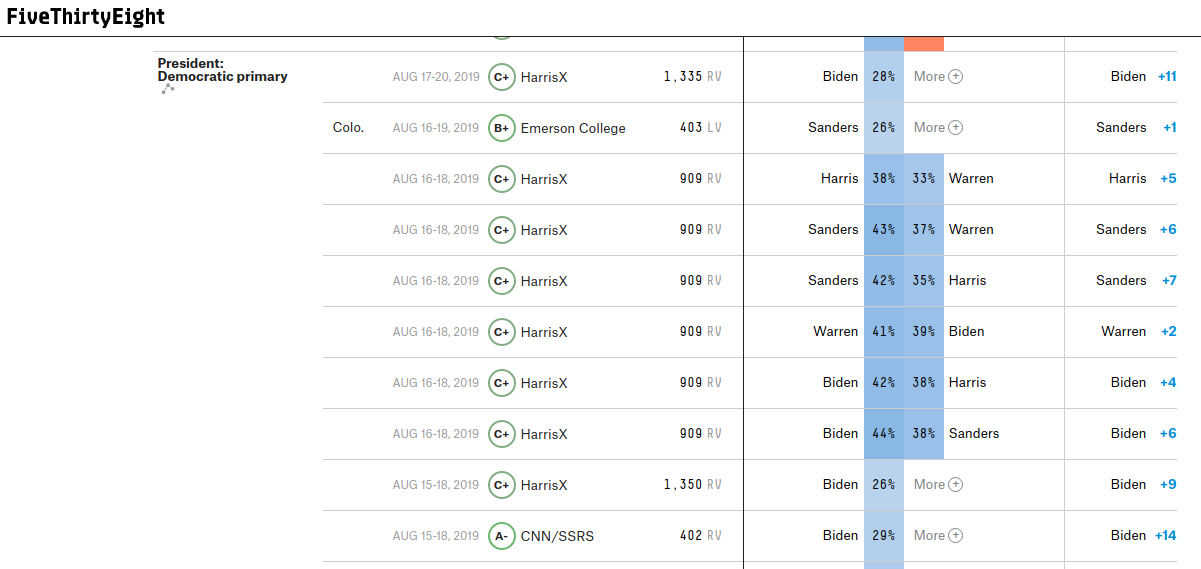
\includegraphics[width=\textwidth]{./pics/cycle-2019-dem-primary.png}
\end{frame}
\begin{frame}[label={sec:org66e41e1}]{Elección primaria 2020}
\flushright
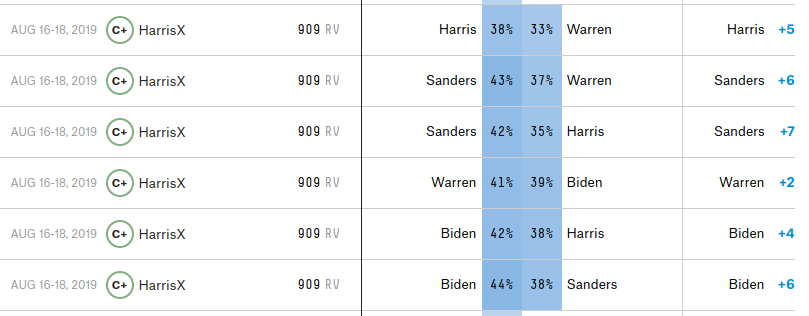
\includegraphics[width=.95\textwidth]{./pics/cycle-2019-dem-primary-zoom.png}
\end{frame}
\begin{frame}[label={sec:orgb8a1321}]{Elección primaria 2020}
\flushright
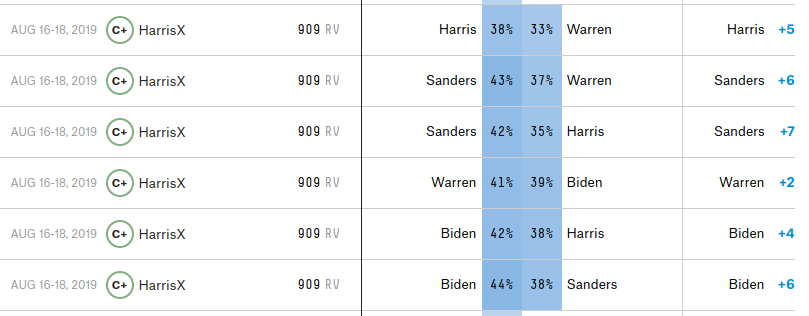
\includegraphics[width=.95\textwidth]{./pics/cycle-2019-dem-primary-zoom.png} \\[0pt]
\bigskip \centering
\color{black}\(Biden \stackrel{\mathclap{\tiny\mbox{+2}}}{<} 
             Warren \stackrel{\mathclap{\tiny\mbox{+5}}}{<} 
             Harris \stackrel{\mathclap{\tiny\mbox{+7}}}{<} 
             Sanders \stackrel{\mathclap{\tiny\mbox{+6}}}{<} 
             Biden\) \\[0pt]
\bigskip
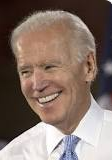
\includegraphics[height=1.5cm]{./pics/biden.png} \(\rightarrow\)

\includegraphics[height=1.5cm]{./pics/warren.png} \(\rightarrow\)
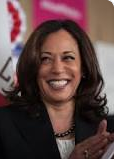
\includegraphics[height=1.5cm]{./pics/harris.png} \(\rightarrow\)

\includegraphics[height=1.5cm]{./pics/sanders.png} \(\rightarrow\)
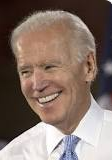
\includegraphics[height=1.5cm]{./pics/biden.png} \(\rightarrow \ldots\)
\end{frame}
\begin{frame}[label={sec:org48671a3}]{Dos interpretaciones del voto}
\begin{columns}
\begin{column}{0.6\columnwidth}
¿Qué busca y consigue una votación?

¿qué significa el resultado?
\end{column}

\begin{column}{0.4\columnwidth}
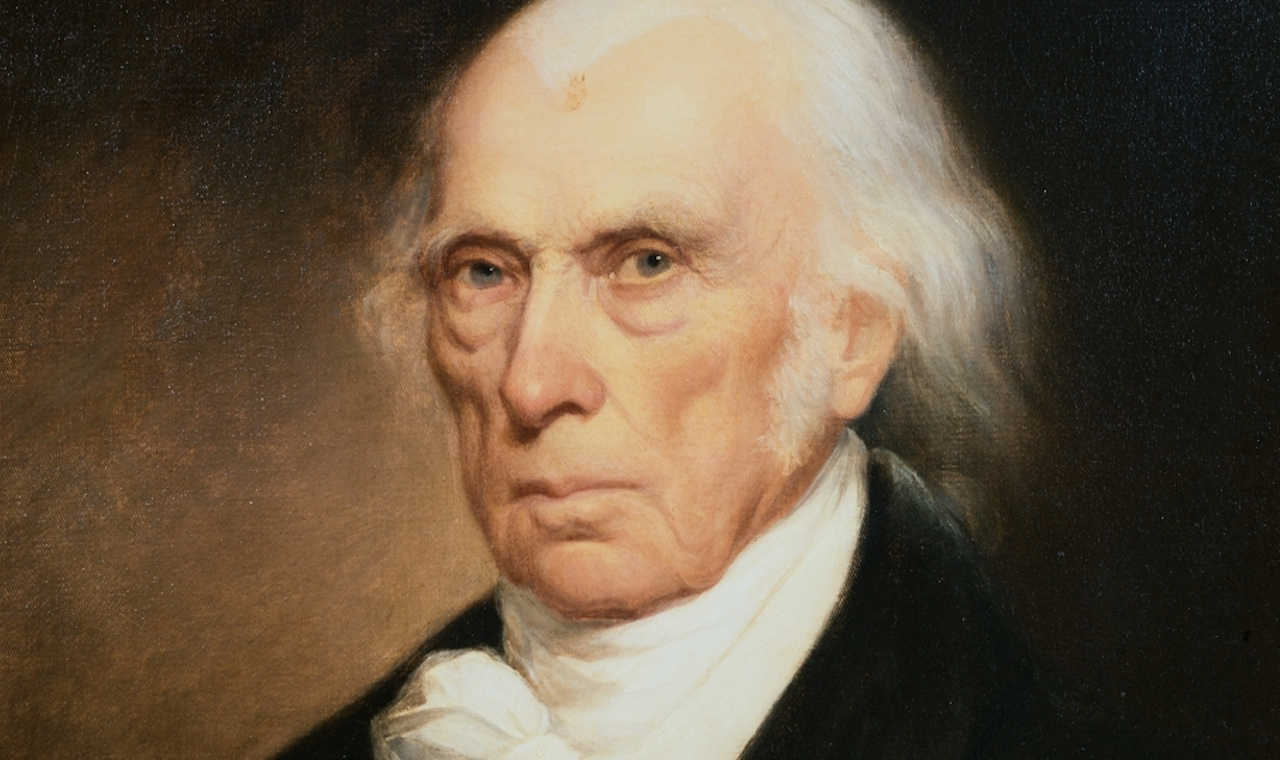
\includegraphics[width=3cm]{./pics/madison.jpg}


\bigskip \pause
\end{column}
\end{columns}
\begin{block}{1. Postura liberal/madisoniana}
\begin{itemize}
\item función = control
\begin{itemize}
\item elecciones periódicas permiten echar a los pillos
\item ley de reacciones anticipadas
\end{itemize}
\item agnóstica sobre el significado
\item separación del poder es precaución secundaria para preservar la libertad
\end{itemize}
\end{block}
\end{frame}
\begin{frame}[label={sec:orgbbb1839}]{Dos interpretaciones del voto}
\begin{columns}
\begin{column}{0.6\columnwidth}
¿Qué busca y consigue una votación?

¿qué significa el resultado?
\end{column}

\begin{column}{0.4\columnwidth}
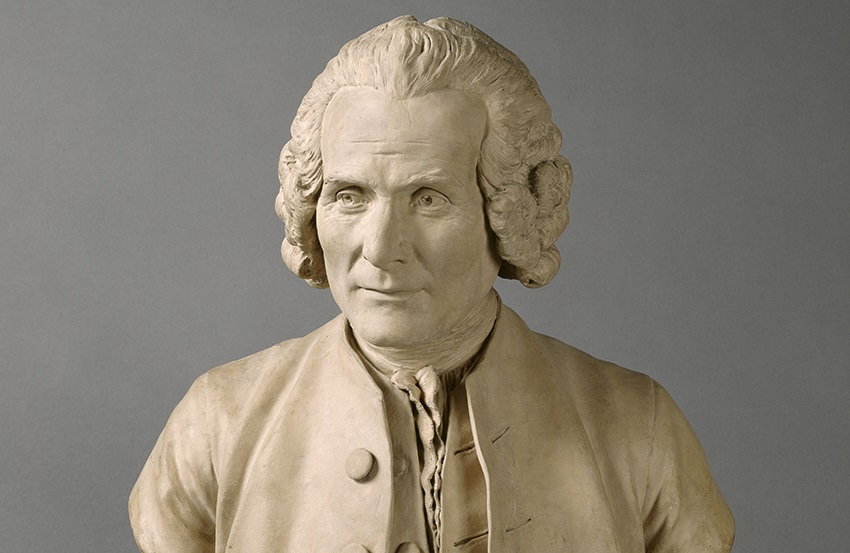
\includegraphics[width=3cm]{./pics/rousseau.jpg}
\bigskip
\end{column}
\end{columns}
\begin{block}{2. Postura populista/rousseauviana}
\begin{itemize}
\item significado = realización de la voluntad general
\begin{itemize}
\item soberano (colectividad) tiene voluntad
\item libertad es obedecer leyes que nos hemos prescrito
\end{itemize}
\item función = consultar para descubrirla
\end{itemize}
\end{block}
\end{frame}
\begin{frame}[label={sec:orgec04934}]{Revisionismo}
Sin importar sus ideales particulares, toda teoría democrática usa \alert{resúmenes sociales} de la decisión de los individuos \\[0pt]
\bigskip
\emph{Social choice} plantea dudas fundamentales acerca del \alert{resumen}, \\[0pt]
quizás obligue a un replanteamiento de la teoría democrática
\bigskip \pause
\begin{itemize}
\item es común quejarnos de la representación, partidos, resultados\ldots{}
\item y muy raro hacerlo de la institución de la \alert{votación}
\item Razón: poca/nula evidencia de que pudiera haber ganado otra opción preferible para la mayoría \\[0pt]
\end{itemize}
\begin{block}{Riker elabora su argumento mostrando dicha la posibilidad}
\centering
\((\Delta \text{resultados} \;|\; \overline{\text{preferencias}})\)
\end{block}
\end{frame}

\begin{frame}[label={sec:org3f60498}]{Formalización de Condorcet}
Premisas
\begin{enumerate}
\item \alert{Preferencia} 
\begin{itemize}
\item \(x,y,z,\ldots\;\) alternativas
\item \(x\;<_i\;y\;\;\) o \(\;\;y\;<_i\;x\;\;\) (o \(\;\;x\;=_i\;y\))
\item La relación \(<_i\) es transitiva: \\[0pt]
\(x\;<_i\;y  \;\;\;\&\;\;\; y\;<_i\;z \;\; \rightarrow \;\; x\;<_i\;z\)
\end{itemize}
\item \alert{Regla de decisión}
\begin{itemize}
\item Sociedad de \(n\) personas (impar)
\item ``\(<\)'' es la elección social
\begin{itemize}
\item (si no se aclara, se sobre-entiende ``por \uline{mayoría''})
\end{itemize}
\end{itemize}
\end{enumerate}
\end{frame}
\begin{frame}[label={sec:org9099d41}]{Formalización de Condorcet}
Si \(n=1,2,3\) y \(X=x,y,z\)

\begin{columns}
\begin{column}{0.4\columnwidth}
\centering
\begin{center}
\begin{tabular}{lll}
1 & 2 & 3\\[0pt]
\hline
x & y & z\\[0pt]
y & z & x\\[0pt]
z & x & y\\[0pt]
\end{tabular}
\end{center}
\end{column}
\begin{column}{0.6\columnwidth}
\begin{itemize}
\item \(y < x\)
\item \(z < y\)
\item \(x < z\)
\end{itemize}

\bigskip \pause
\end{column}
\end{columns}
\begin{block}{Si impusiéramos transitividad tb impondríamos un dictador}
\begin{description}
\item[{Si consultamos que}] \(z < y < x\)
\end{description}

\begin{description}
\item[{y por economía inferimos}] \(z < x\)
\item[{convertiríamos a 1 en \uline{dictadora}}] (sólo ella \(z <_1 x\))
\end{description}
\bigskip \pause
\end{block}
La teoría democrática: 
\includegraphics[width=1cm]{./pics/emoji-panic.png} 
\end{frame}
\begin{frame}[label={sec:org2759837}]{Ingredientes para un meme}
\begin{columns}
\begin{column}{0.5\columnwidth}

\includegraphics[width=.85\textwidth]{./pics/kids-in-pool-meme.jpg} 
\end{column}
\begin{column}{0.5\columnwidth}
mamá = teoría política 

hija = transitividad 

hijo = no-dictadura 

calaca = teoría democrática
\end{column}
\end{columns}
\end{frame}
\section{Los estudios contrafactuales de Riker}
\label{sec:orgac961f9}
\begin{frame}[label={sec:org49f4825}]{Presidentes minoritarios en EE.UU.}
\scriptsize \centering
\begin{center}
\begin{tabular}{lrlrrr}
 & Año & Ganador & voto & margen & 3er\\[0pt]
\hline
\(a\) & 1824 & Adams Jr & 31.0 & \(-10.3\) & 13.0\\[0pt]
\(b\) & 44 & Polk & 49.6 & 1.5 & 2.3\\[0pt]
\(c\) & 48 & Taylor & 47.3 & 4.8 & 10.1\\[0pt]
\hline
\(d\) & 56 & Buchanan & 45.3 & 12.2 & 21.5\\[0pt]
\(e\) & 60 & Lincoln & 39.8 & 10.3 & 18.1\\[0pt]
\(f\) & 80 & Garfield & 48.3 & 0.02 & 3.3\\[0pt]
\hline
\(g\) & 84 & Cleveland & 48.5 & 0.2 & 1.7\\[0pt]
\(h\) & 88 & Harrison & 47.8 & \(-0.8\) & 2.2\\[0pt]
\(i\) & 92 & Cleveland & 46.0 & 3.0 & 8.5\\[0pt]
\hline
\(j\) & 1912 & Wilson & 41.8 & 14.4 & 23.6\\[0pt]
\(k\) & 16 & Wilson & 49.2 & 3.1 & 3.2\\[0pt]
\(l\) & 48 & Truman & 49.5 & 4.4 & 2.4\\[0pt]
\hline
\(m\) & 60 & Kennedy & 49.7 & 0.2 & 0.2\\[0pt]
\(n\) & 68 & Nixon & 43.4 & 0.7 & 13.5\\[0pt]
\(o\) & 92 & Clinton & 43.0 & 6.6 & 18.9\\[0pt]
\hline
\(p\) & 96 & Clinton & 49.2 & 8.5 & 8.4\\[0pt]
\(q\) & 2000 & Bush Jr & 47.9 & \(-0.5\) & 2.7\\[0pt]
\(r\) & 16 & Trump & 46.1 & \(-2.1\) & 3.3\\[0pt]
\end{tabular}
\end{center}
Contraste: (1) colegio electoral (2) pluralidad (3) segunda vuelta
\end{frame}
\begin{frame}[label={sec:org04aeec7}]{Francia 2002}
\centering   
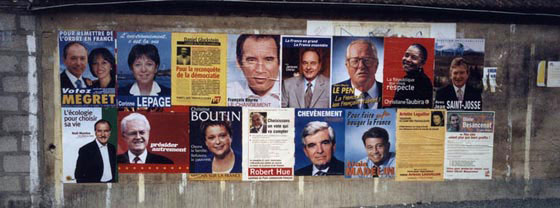
\includegraphics[width=\textwidth]{./pics/Affiches-premier-tour2002.jpg}
\end{frame}
\begin{frame}[label={sec:org158fa54}]{Francia 2002}
\begin{columns}
\begin{column}{0.33\columnwidth}
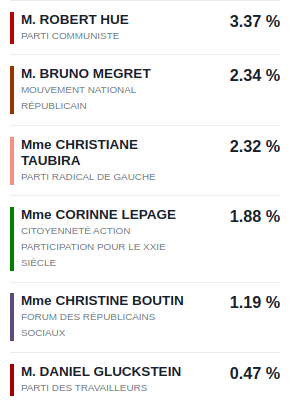
\includegraphics[width=\textwidth]{./pics/f3.png}
\end{column}
\begin{column}{0.33\columnwidth}
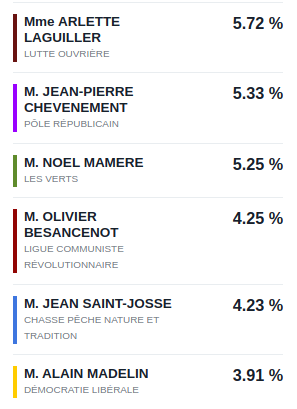
\includegraphics[width=\textwidth]{./pics/f2.png}
\end{column}
\begin{column}{0.33\columnwidth}
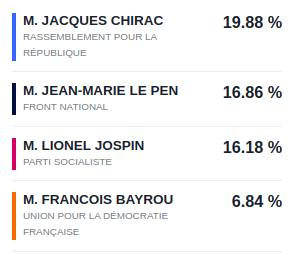
\includegraphics[width=\textwidth]{./pics/f1.png}
\end{column}
\end{columns}

\pause \centering
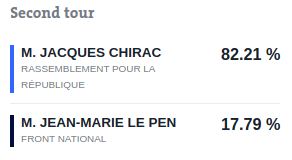
\includegraphics[width=.33\textwidth]{./pics/f4.png}
\end{frame}
\begin{frame}[label={sec:org576ef01}]{Francia 2002: intención \(2^a\) \emph{vs} voto \(1^a\)}
\centering   
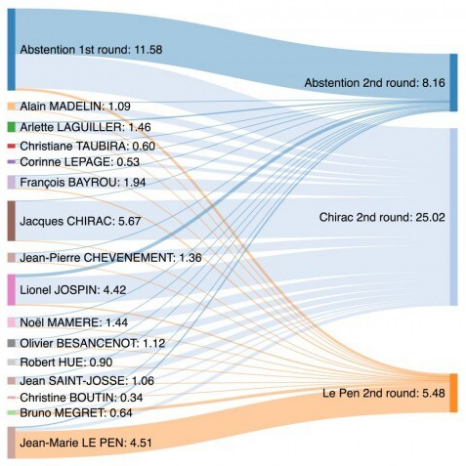
\includegraphics[width=.7\textwidth]{./pics/f1-2.png}
\end{frame}
\begin{frame}[label={sec:orge8dbf63}]{Las sondas Voyager}
\begin{columns}
\begin{column}{0.6\columnwidth}
\begin{itemize}
\item Lanzadas al espacio en 1977
\item Afortunada alineación planetaria para visitar gigantes exteriores
\item Gravedad planetaria los impulsa fuera del sistema solar
\item \href{https://www.youtube.com/watch?v=niKWI1AFMno}{\ExternalLink Carl Sagan}
\item \href{https://www.youtube.com/watch?v=MGPM58S5Njg}{\ExternalLink Voyager 2 alcanza el espacio interestelar en 2012}
\end{itemize}
\end{column}
\begin{column}{0.4\columnwidth}
\centering
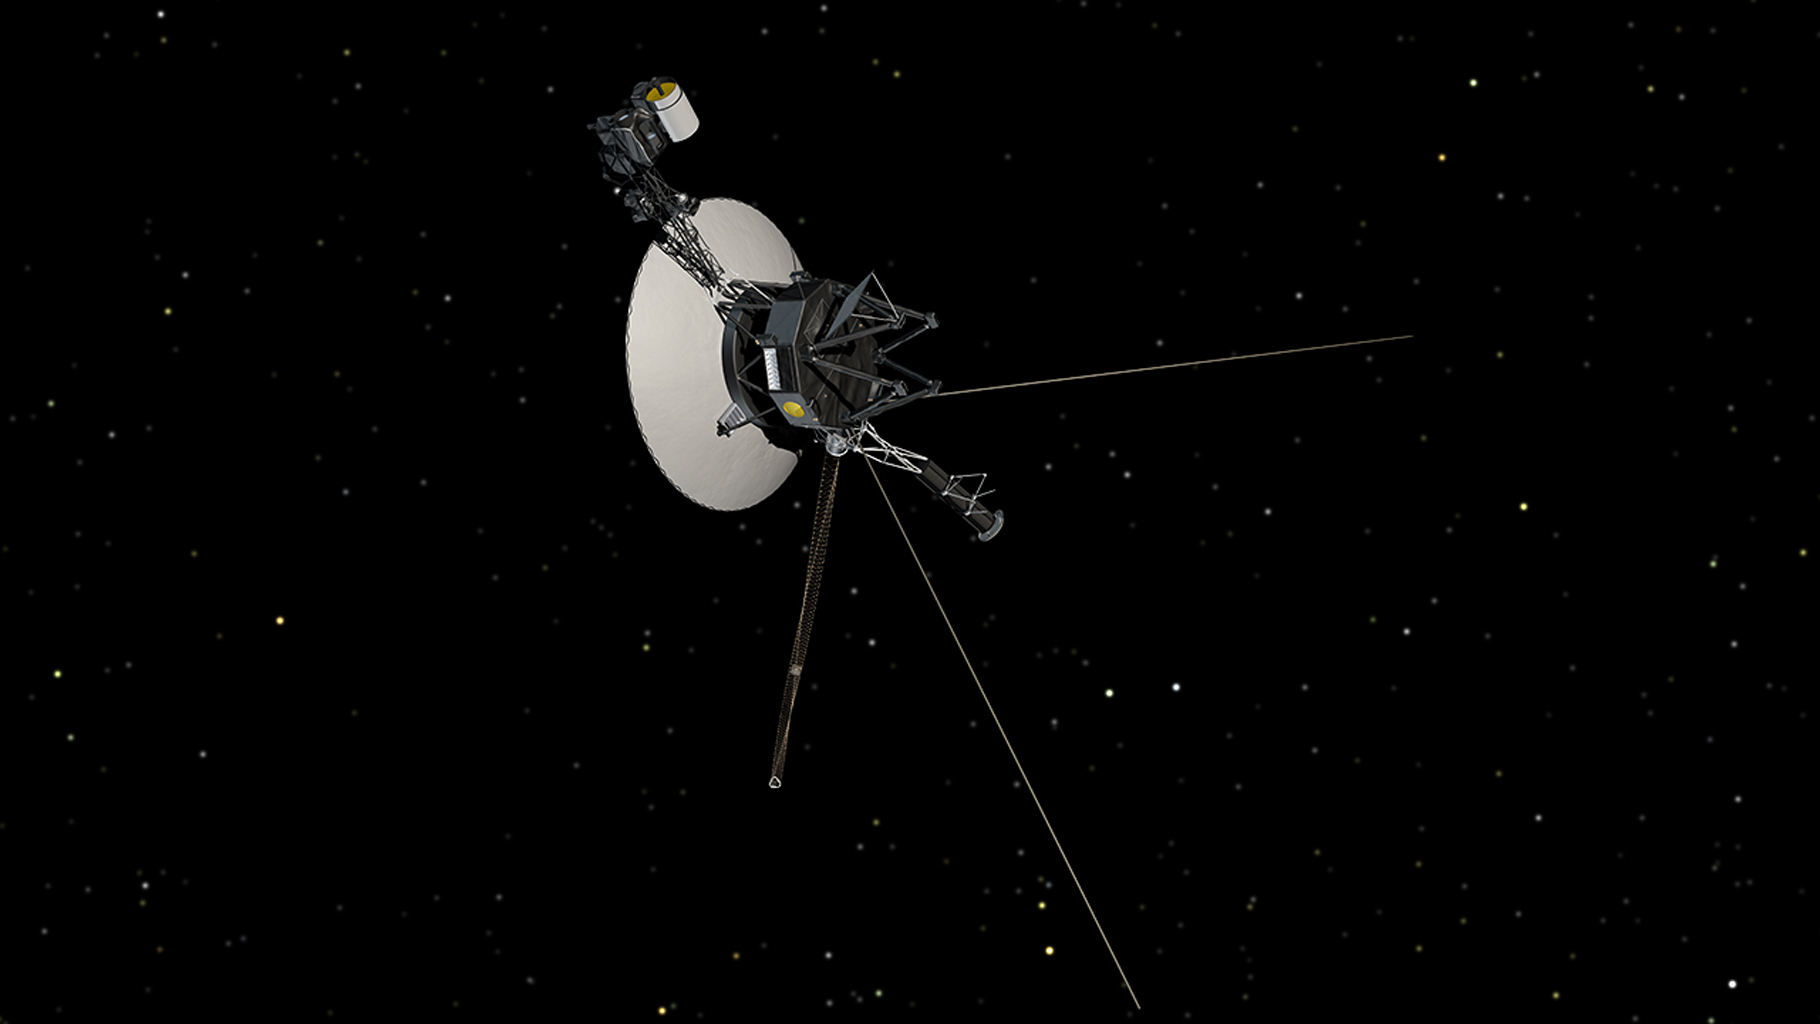
\includegraphics[width=\textwidth]{./pics/voyager1.jpg} \\[0pt]
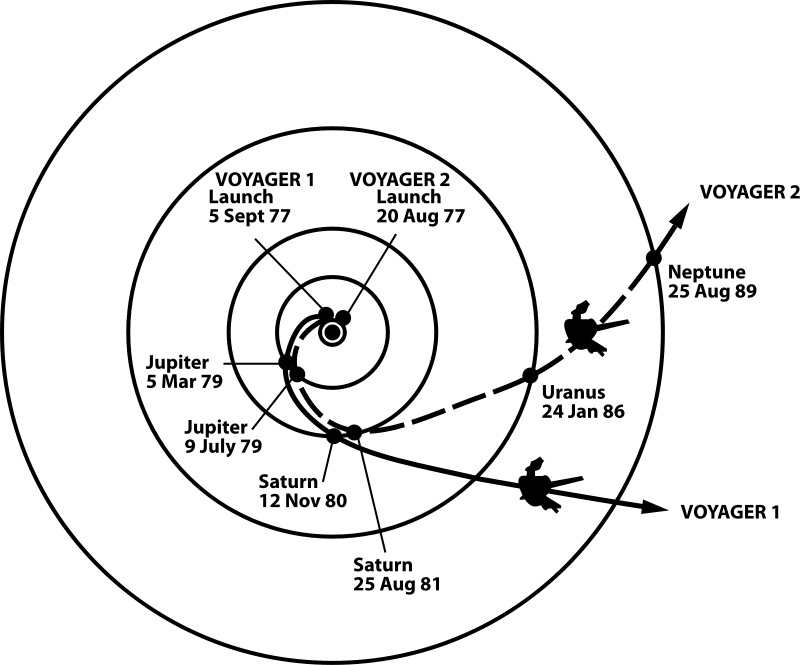
\includegraphics[width=\textwidth]{./pics/800px-Voyager_Path.svg.png}
\end{column}
\end{columns}
\end{frame}
\begin{frame}[label={sec:org0e8f9ab}]{Preparativos}
\begin{columns}
\begin{column}{0.6\columnwidth}
\begin{itemize}
\item Tras consultar 80 astrónomos \emph{Jet Propulsion Lab} seleccionó 32 pares de trayectorias factibles
\item Faltaba determinar el valor científico de las trayectorias
\item 10 equipos de especialistas las ordenaron (p.ej. MAG = campos magnéticos, IRIS = radiación infrarroja\(\ldots\))
\item Reunión presencial para obtener utilidad \emph{cardinal}
\item \href{https://voyager.jpl.nasa.gov/mission/timeline/\#event-the-first-science-meeting}{\ExternalLink Línea de tiempo}
\end{itemize}
\end{column}
\begin{column}{0.4\columnwidth}
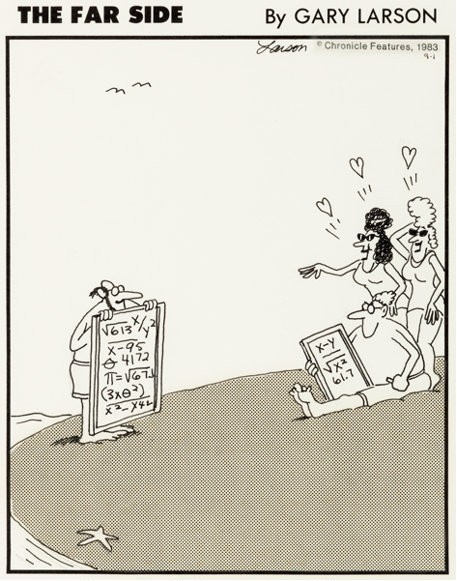
\includegraphics[width=\textwidth]{./pics/larson3.jpeg}
\end{column}
\end{columns}
\end{frame}
\begin{frame}[label={sec:org7128542}]{Preparativos}
\centering
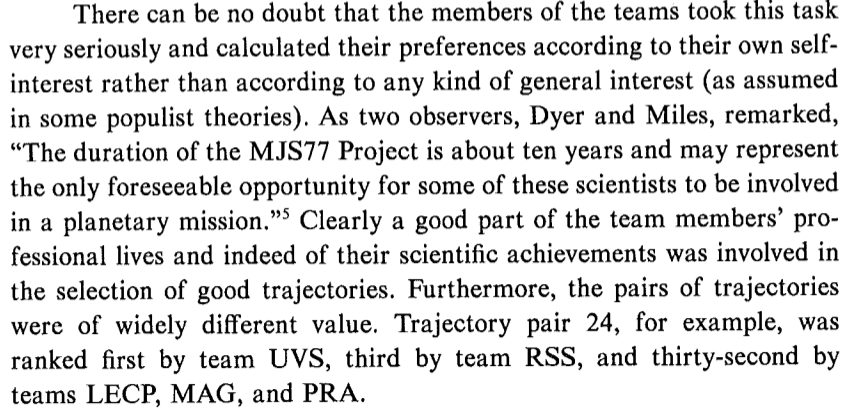
\includegraphics[width=\textwidth]{./pics/rk1.png}
\end{frame}
\begin{frame}[label={sec:org0be7064}]{Preparativos}
\centering
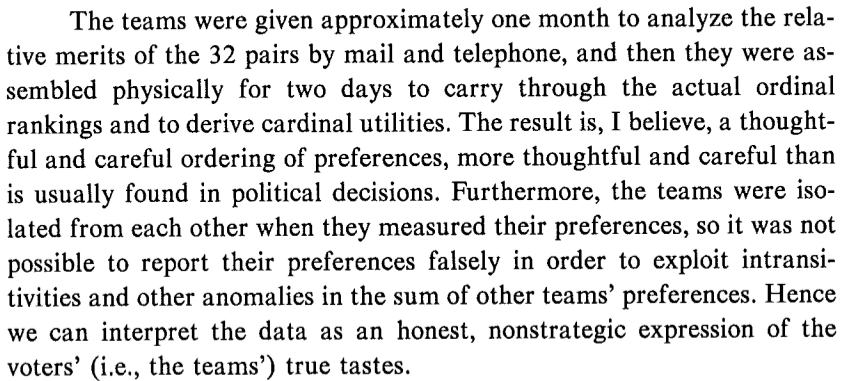
\includegraphics[width=\textwidth]{./pics/rk2.png}
\end{frame}
\begin{frame}[<+->][label={sec:org6949743}]{Inferencia de utilidad cardinal}
\begin{block}{Von Neumann-Morgenstern vía experimental}
\begin{enumerate}
\item Sujeto ordena tres alternativas: \(a,b,c\)
\item Fijas \(u(a)=1\;\&\;u(c)=0\)
\item Ofreces al sujeto lotería \(L(p)\) ó \(b\) \\[0pt]
con las ganancias siguientes:
\begin{itemize}
\item \(Eu(L) = pu(a) + (1-p)u(c) = p\)
\item ó \(u(b)\)
\end{itemize}
\item Empiezas con \(p=1\) para que prefiera \(L\) sobre \(b\)
\item Reduces gradualmente \(p\) hasta que surja indiferencia
\item \((p|\text{indif})\) es la utilidad cardinal de \(b\)
\end{enumerate}
\end{block}
\end{frame}
\begin{frame}[label={sec:orgf7da155}]{Cuatro métodos}
\begin{center}
\begin{tabular}{lll}
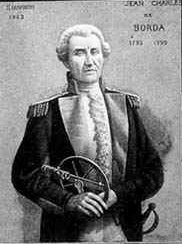
\includegraphics[width=.25\textwidth]{./pics/borda.jpg} & 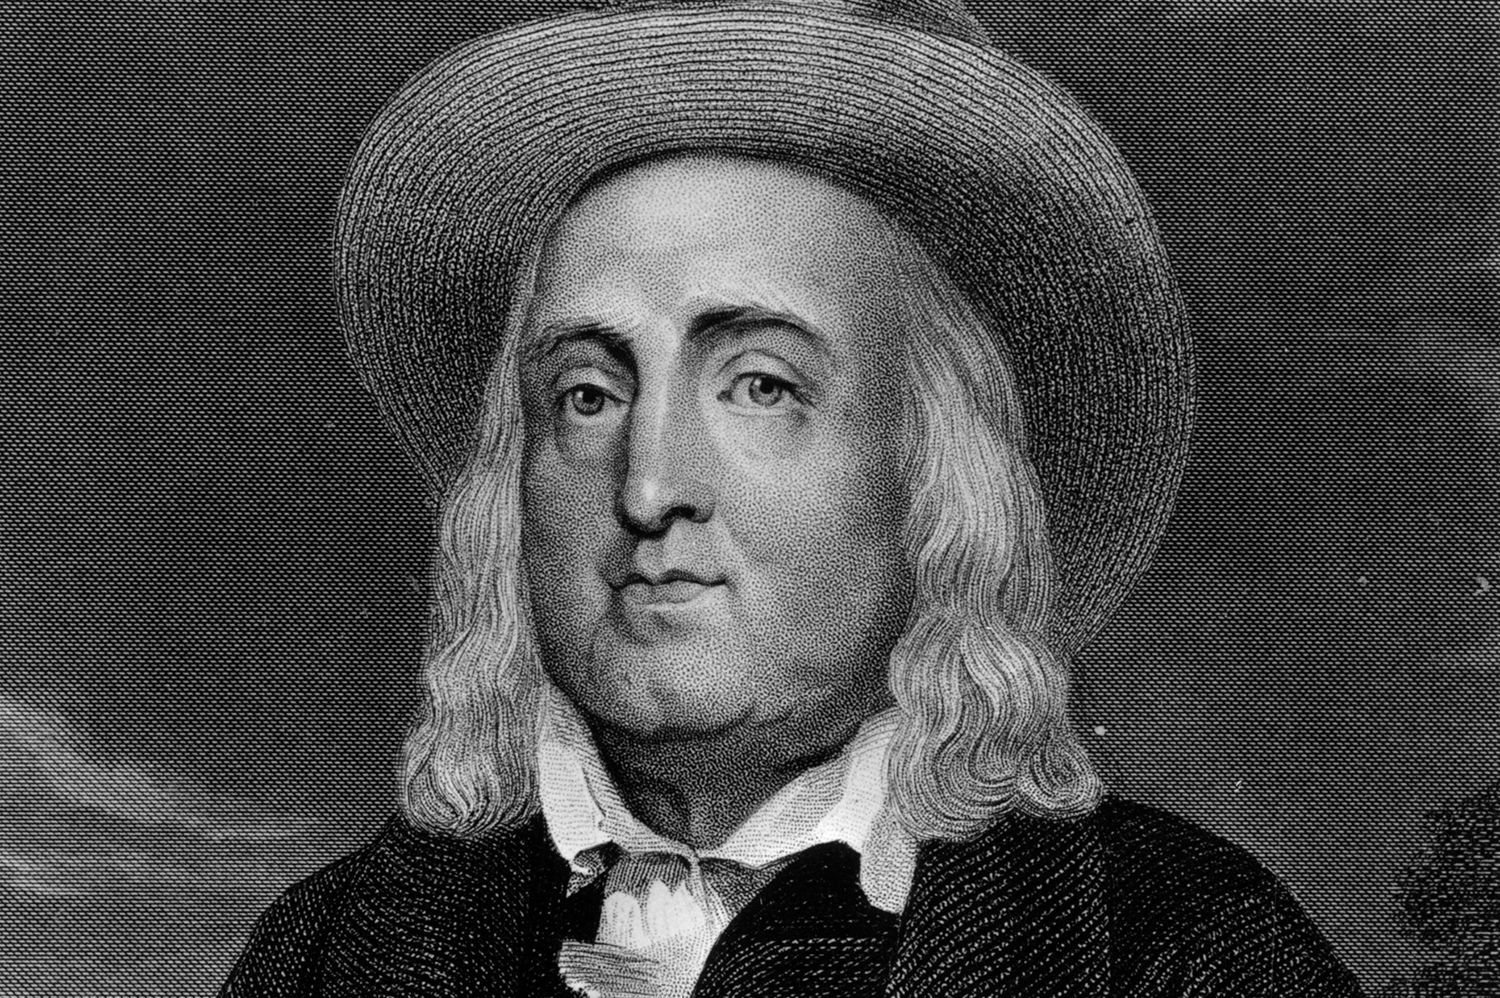
\includegraphics[width=.25\textwidth]{./pics/bentham.jpg} & 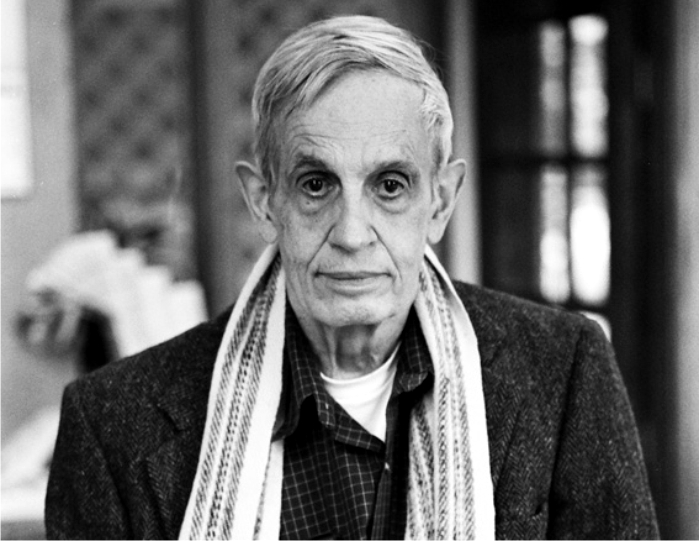
\includegraphics[width=.25\textwidth]{./pics/nash.jpg}\\[0pt]
\tiny{Jean-Charles de Borda} & \tiny{Jeremy Bentham} & \tiny{John Nash}\\[0pt]
\tiny{(1733--1799)} & \tiny{(1748--1832)} & \tiny{(1928--2015)}\\[0pt]
\end{tabular}
\end{center}

\begin{enumerate}
\item Suma de puntos ordinales (Borda)
\item Suma de valores cardinales (Bentham)
\item Multiplicación de valores cardinales (Nash)
\item Comparaciones pareadas (Condorcet)
\end{enumerate}
\end{frame}
\begin{frame}[label={sec:org9672bfc}]{Cuatro métodos}
\centering
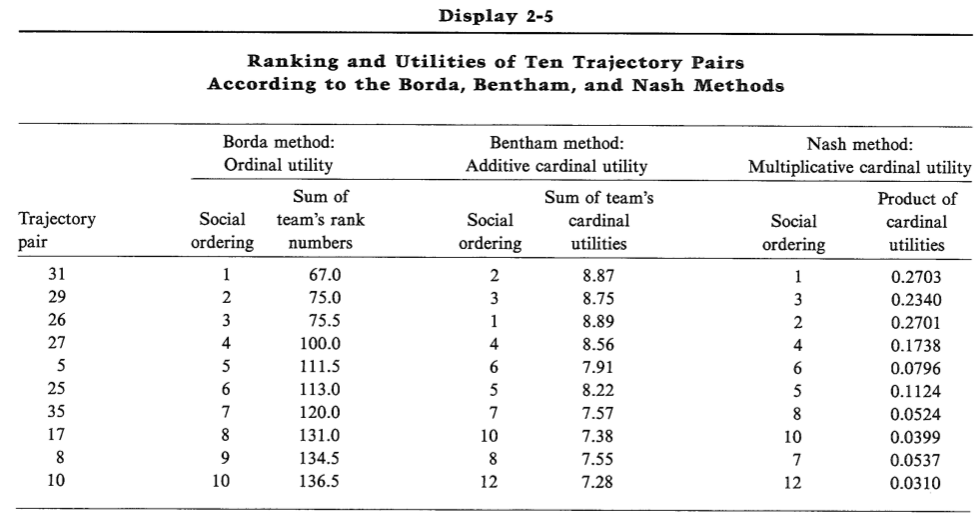
\includegraphics[width=\textwidth]{./pics/rk3.png}
\end{frame}
\begin{frame}[label={sec:org9516581}]{Cuatro métodos: Hay ganador Condorcet}
\centering
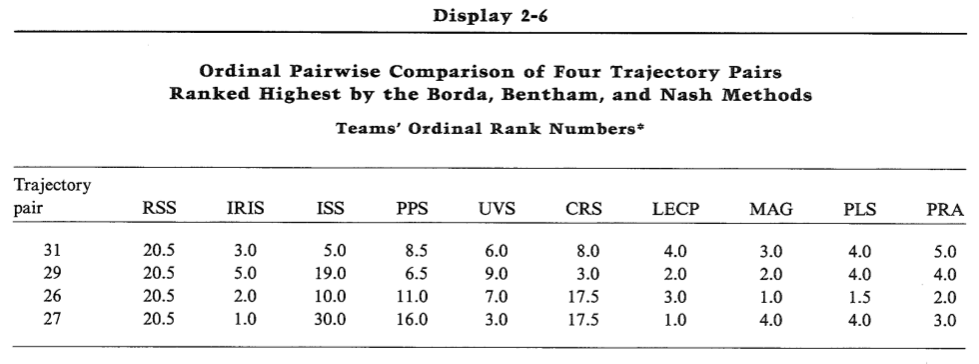
\includegraphics[width=\textwidth]{./pics/rk4.png} \\[0pt]
\pause
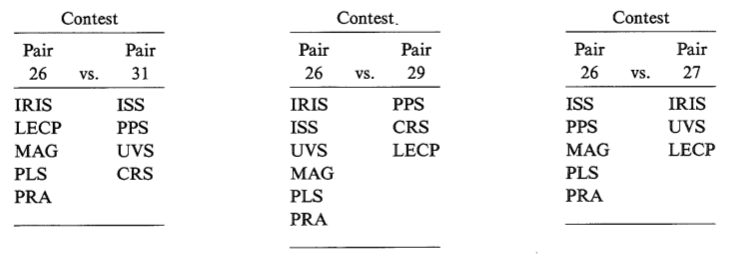
\includegraphics[width=\textwidth]{./pics/rk5.png}
\end{frame}
\begin{frame}[label={sec:org204caba}]{Desenlace}
\begin{block}{En Pasadena}
\begin{itemize}
\item seleccionaron 26' (modificada)
\item ganador Condorcet/Bentham
\item quienes notaron que 31' también habría ganado no lograron convencer\(\ldots\)
\end{itemize}
\end{block}
\centering
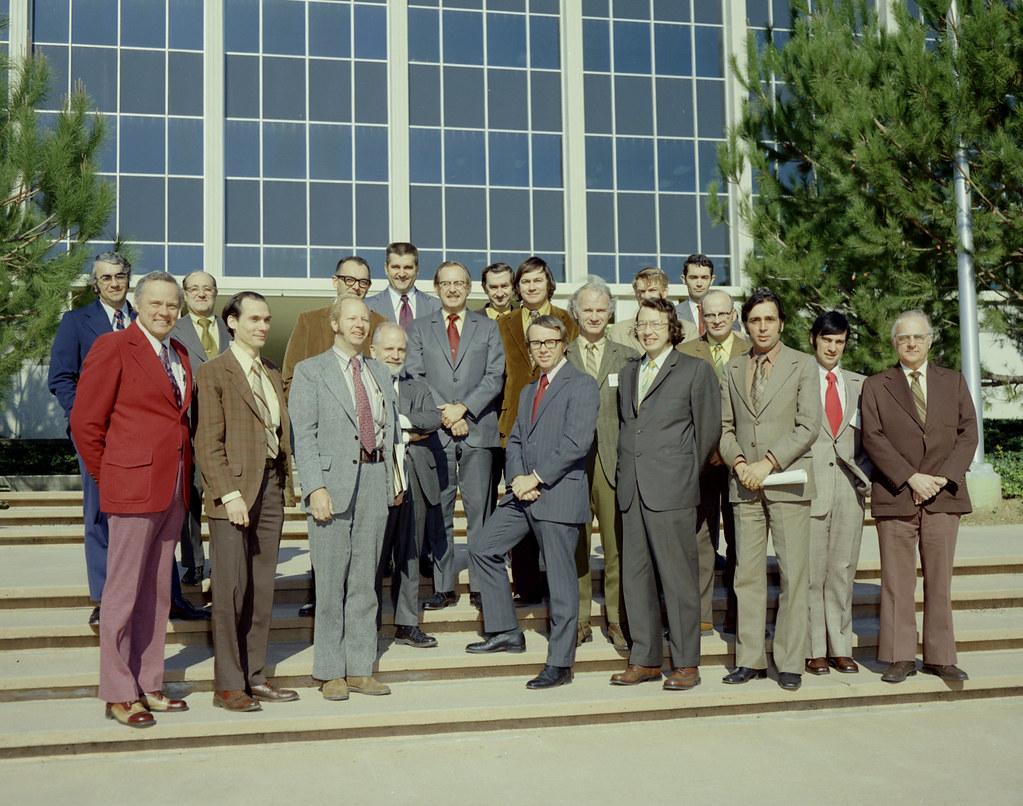
\includegraphics[width=.6\textwidth]{./pics/jpl-oct-1973.jpg} \\[0pt]
\end{frame}
\begin{frame}[label={sec:org3f1943e}]{Un caso (abstracto) que desconcierta}
\begin{center}
\begin{tabular}{lllll}
 &  & votante &  & \\[0pt]
1 & 2 & 3 & 4 & 5\\[0pt]
\hline
\(a\) (1.00) & \(d\) (1.00) & \(e\) (1.00) & \(b\) (1.00) & \(b\) (1.00)\\[0pt]
\(d\) (0.90) & \(a\) (0.61) & \(c\) (0.80) & \(d\) (0.90) & \(e\) (0.96)\\[0pt]
\(b\) (0.60) & \(b\) (0.60) & \(a\) (0.70) & \(a\) (0.75) & \(c\) (0.70)\\[0pt]
\(c\) (0.55) & \(e\) (0.59) & \(b\) (0.55) & \(e\) (0.74) & \(a\) (0.60)\\[0pt]
\(e\) (0.50) & \(c\) (0.50) & \(d\) (0.50) & \(c\) (0.50) & \(d\) (0.50)\\[0pt]
\end{tabular}
\end{center}
\pause 
\begin{columns}
\begin{column}{0.4\columnwidth}
\begin{block}{Ganador}
\begin{itemize}
\item Condorcet = \(a\)
\item Borda = \(b\)
\item Pluralidad = \(b\)
\item Bentham = \(d\)
\item Nash = \(e\)
\end{itemize}
\end{block}
\end{column}
\begin{column}{0.4\columnwidth}
Excepto \(c\), cada opción puede ganar con alguno de los métodos
\end{column}
\end{columns}
\end{frame}
\begin{frame}[label={sec:orge48ebae}]{Un caso (abstracto) que desconcierta}
\begin{block}{Aspiración democrática}
\centering
\(\text{Resultado} = f(\text{gustos})\)
\end{block}
\begin{block}{En la práctica es una función bivariada}
\centering
\(\text{Resultado} = f(\text{gustos}, \text{método})\)
\end{block}
\pause \bigskip
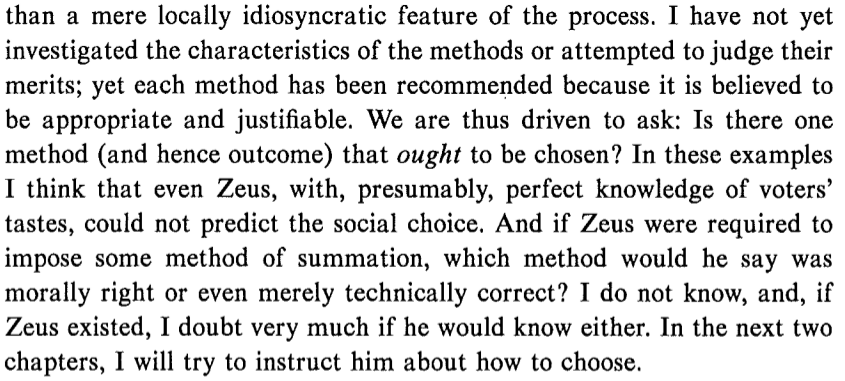
\includegraphics[width=\textwidth]{./pics/rk7.png}
\end{frame}
\section{Elección presidencial de 2018}
\label{sec:org2051c22}
\begin{frame}[label={sec:org532b012}]{El cheque en blanco}
\centering

\includegraphics[width=.2\textwidth]{./pics/atto-titu.jpeg}

\includegraphics[width=.8\textwidth]{./pics/at1-2.png}

\bigskip
¿Existe el \alert{mandato de la mayoría}?
\end{frame}
\begin{frame}[label={sec:orgb212461}]{¿Por qué votaste por AMLO?}
\begin{block}{El ``mandato'' de la mayoría}
\begin{itemize}
\item Mito muy socorrido/generalizado: que el triunfo confiere al ganador un mandato popular en apoyo de su programa
\item Andrew Jackson en su mensaje inaugural al Congreso 1829: ``no hay más impedimentos para la libre operación de la voluntad pública''
\item AMLO en Zócalo 2018: ``Una mayoría importante ha decidido iniciar la cuarta transformación de la vida pública de México''
\end{itemize}

\pause \bigskip
\end{block}
\begin{columns}
\begin{column}{0.6\columnwidth}
Pasa por alto que se vota por toda clase de razones, contradictorias incluso en el propio votante
\end{column}
\end{columns}
\end{frame}

\begin{frame}[label={sec:org1121ebd}]{¿Por qué votaste por AMLO?}
\begin{columns}
\begin{column}{.5\columnwidth}
\begin{itemize}
\item muerte al neoliberalismo
\item justicia social
\item acabará la corrupción
\item la inseguridad
\item es nacionalista
\item cambio necesario
\item es de izquierda
\item por enojo
\item por amor
\item porque es cristiano
\item \(\ldots\)
\end{itemize}
\end{column}
\begin{column}{.1\columnwidth}
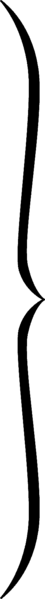
\includegraphics[height=.9\textheight]{./pics/accolade.png}
\end{column}
\begin{column}{.4\columnwidth}
\(53\% \approx 30\) millones
\end{column}
\end{columns}
\end{frame}
\begin{frame}[<+->][label={sec:org9168415}]{Encuesta post-electoral 12 julio 2018}
\begin{block}{¿Por quién votó usted para Presidente de la República?}
\begin{center}
\begin{tabular}{rrr}
Contestó & No contestó & N\\[0pt]
\hline
1032 & 396 & 1428\\[0pt]
\end{tabular}
\end{center}
\end{block}
\begin{block}{Quitando NRs y credencial sin marca}
\begin{center}
\begin{tabular}{rrrrr}
AMLO & Anaya & Meade & Bronco & N\\[0pt]
\hline
0.68 & 0.17 & 0.12 & 0.03 & 1010\\[0pt]
\end{tabular}
\end{center}
\end{block}
\begin{block}{No hay pregunta \emph{¿por qué votó por x?}}
En vez, hay \emph{termómetros} \\[0pt]
(y supondremos que guardan alguna relación con el \emph{porqué})
\end{block}
\end{frame}
\begin{frame}[label={sec:org042fa7c}]{Votantes AMLO (\(N = 684\))}
\begin{block}{Termómetros}
\centering
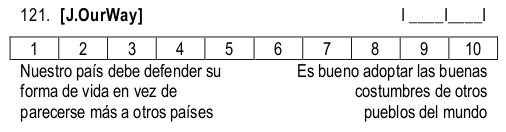
\includegraphics[height=1.5cm]{./pics/q121.png}
\footnotesize
\begin{center}
\begin{tabular}{llll}
1--3 &  &  & 8--10\\[0pt]
\hline
39\% & Defender modo de vida & Adoptar bueno de otros & 31\%\\[0pt]
48\% & Evitar el conflicto & Conflicto inevitable & 20\%\\[0pt]
48\% & Religión no se impone & Religión como base leyes & 19\%\\[0pt]
29\% & Redistribución & Iniciativa individual & 36\%\\[0pt]
52\% & Medio ambiente & Crecimiento económico & 19\%\\[0pt]
46\% & Migrantes bienvenidos & No son bienvenidos & 20\%\\[0pt]
25\% & \emph{Pro choice} & \emph{Pro life} & 45\%\\[0pt]
22\% & Más servicios públicos & Menos impuestos & 43\%\\[0pt]
\end{tabular}
\end{center}
\end{block}
\end{frame}

\begin{frame}[label={sec:org87b2226}]{Otros sistemas}
\begin{block}{La votación cuadrática}
\begin{itemize}
\item El votante tiene un prespupuesto de créditos (100)
\item Vota a favor de una alternativa, en contra, o se abstiene
\item Los votos cuestan créditos
\item Puede acumular votos en favor/contra de una alternativa, pero cada voto extra cuesta más créditos que el anterior:
\end{itemize}
\begin{center}
\begin{tabular}{rr}
votos & créditos\\[0pt]
\hline
1 & 1\\[0pt]
2 & 4\\[0pt]
3 & 9\\[0pt]
\ldots{} & \\[0pt]
\end{tabular}
\end{center}
Ejercicio: \url{https://bit.ly/3Tb8mo6}
\end{block}
\end{frame}
\section{Generalización de Arrow}
\label{sec:org8639346}
\begin{frame}[label={sec:orgd2e8c28}]{Arrow}
\begin{block}{Imposible cumplir 6 \emph{desiderata}}
\begin{enumerate}
\item \(>2\) alternativas
\item Dominio irrestricto
\item No dictadura
\item Principio de Pareto: \(x>y\) cuando \(x>_iy\;\forall i\)
\item IIA: la pref. colectiva entre 2 alternativas nunca depende de las pref. individuales respecto de otra(s) alternativa(s)
\item Transitividad
\end{enumerate}
\end{block}
\end{frame}

\begin{frame}[label={sec:orged19179}]{Independencia de alternativas irrelevantes}
\begin{block}{Ilustración de violación (individual) de IIA}
Quieres postre. El mesero ofrece nieve de guanábana o brownie. Ordenas nieve. Vuelve el mesero y anuncia que también le queda dulce de mamey. Dices ``entonces quiero brownie'' (en vez de nieve o mamey)
\pause
\end{block}
\begin{block}{Fácil incumplirla colectivamente}
\begin{itemize}
\item (7 personas) Blanca \(>_i\) Clara  \(>_i\) Aura
\item (6 personas) Clara  \(>_i\) Aura   \(>_i\) Blanca
\item (5 personas) Aura   \(>_i\) Blanca \(>_i\) Clara
\end{itemize}
Pluralidad A \emph{v} B: gana A (11 votos). Entra C, gana B
\pause
\end{block}
\begin{exampleblock}{Lo que pide IRR}
Que si Clara (la candidata irrelevante) entrara, gane Aura o Clara, no Blanca
\end{exampleblock}
\end{frame}

\begin{frame}[label={sec:orgec10fdf}]{La paradoja se generaliza}
Arrow busca las propiedades mínimas de una regla razonablemente democrática
\bigskip
\begin{block}{Schwartz: tan mínimas que las comparten}
\begin{itemize}
\item una democracia constitucional ideal
\item una aristocracia ilustrada
\item una oligarquía corrupta
\item una tiranía sanguinaria
\end{itemize}
\end{block}
\end{frame}

\section{Retorno a la mayoría: teorema de May}
\label{sec:orgfe27663}
\begin{frame}[label={sec:orga26ba19}]{El teorema de May}
Notación de Schwartz
\begin{columns}
\begin{column}{.5\columnwidth}
\begin{block}{Dada una regla de votación}
\begin{description}
\item[{\(x\) derrota \(y\)}] si, cuando sólo \((x,y)\) son factibles, la regla elige \(x\)
\item[{\(x\) empata \(y\)}] cuando ninguna vence a la otra
\end{description}
\bigskip \pause
\end{block}
\end{column}
\begin{column}{.5\columnwidth}
\begin{example}[Regla de mayoría]
\begin{description}
\item[{\(x\) derrota \(y\)}] si \(x\) obtiene más votos que \(y\)
\item[{\(y\) derrota \(x\)}] si \(y\) obtiene más votos que \(x\)
\item[{\(x\) empata \(y\)}] cuando obtienen los mismos votos
\end{description}
\end{example}
\end{column}
\end{columns}
\bigskip
Ojo: otros autores usan otras notaciones (\(x>y\) o \(x\;\text{P}\;y\))
\end{frame}

\begin{frame}[label={sec:org3183690}]{Notación de Schwartz}
\begin{itemize}
\item Con \(n\) votantes
\item que deciden entre dos alternativas, representadas \(-1\) y 1
\item y 0 indica indiferencia/empate
\end{itemize}
\begin{block}{Definiciones}
\begin{itemize}
\item Una \alert{combinación de votos} es un vector \((x_1,...,x_n)\), donde \(x_i\in(-1,0,1)\), que representa un modo en que \(i=1,2,...,n\) pueden votar o abstenerse
\item Cualquier \alert{regla de votación binaria} puede representarse como una función \(f\) de combinaciones de votos donde \(f(x_1,...,x_n)=\begin{cases}-1\\0\\1\end{cases}\)
\end{itemize}
\end{block}
\end{frame}

\begin{frame}[label={sec:org6079a5b}]{Tres propiedades deseables de \(f\)}
\begin{description}[<+->]
\item[{(A) Anonimidad}] trato igualitario de los votantes \(f(x_1,...,x_i,...,x_j,...,x_n) \equiv f(x_1,...,x_j,...,x_i,...,x_n)\)
\item[{(N) Neutralidad}] trato igualitario de las alternativas \(f(x_1,...,x_n) \equiv -f(-x_1,...,-x_n)\)
\item[{(E) Fragilidad de empates}] si \(f(x_1,...,x_n) = 0\) y \((y_1,...,y_n)\) resulta de cambiar uno o más 0s por 1s, con lo demás constante, entonces \(f(y_1,...,y_n) = 1\)
\end{description}
\bigskip \pause
\begin{theorem}[de May]
La de mayoría es la única regla que tiene simultáneamente las propiedades A, N y E 
\end{theorem}
\end{frame}

\begin{frame}[label={sec:org3f3ec57}]{El lugar distinguido entre las reglas de decisión}
\begin{block}{Debido a sus tres propiedades}
parece ``natural'' usar la regla de mayoría con alternativas binarias (aceptar/rechazar mociones, fallos, tasas, planes, \ldots{})
\end{block}

\bigskip \pause
Tan es así, que muchos asocian \alert{democracia} con \alert{mayoritarismo} --- lo cual, veremos, es falso (\emph{cf.} Lijphart, los Federalistas, neo-institucionalismo\ldots{})

\bigskip \pause
\begin{exampleblock}{Tarea: excepciones}
\begin{itemize}
\item ¿Qué instancias reales prescinden del mayoritarismo?
\item CPEUM
\end{itemize}
\end{exampleblock}
\end{frame}

\begin{frame}[label={sec:orgb1068a9}]{Otras reglas binarias}
¿Qué propiedades les faltan?
\begin{itemize}
\item Las encuestas violan la condición (E): si \(f(0,x_2,...,x_n)=0\) pero \(i=1\) no está en la muestra, \(f(1,x_2,...,x_n)\neq1\)
\item La mayoría calificada viola (N)
\item La Junta de Coordinación Política del Congreso viola (A)
\end{itemize}
\end{frame}

\begin{frame}[label={sec:org9dfd0df}]{Democracia \(\neq\) mayoritarismo}
La regla de mayoría: condición necesaria pero \alert{insuficiente} de la democracia

\pause \bigskip
\begin{block}{Separación del poder}
\begin{itemize}
\item Introduce instituciones que complementan/limitan la regla de mayoría
\item La noción central de la ingeniería institucional es \emph{incumplir} una o más de las propiedades (A) (N) y (E)
\end{itemize}
\end{block}
\end{frame}

\section{Recapitulación}
\label{sec:orgd8dc25e}
\begin{frame}[label={sec:orga28f3d9}]{Las interrogantes}
\centering
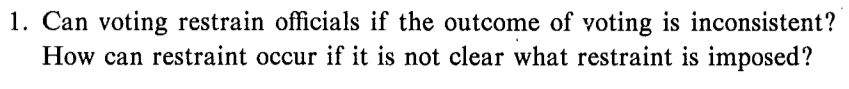
\includegraphics[width=\textwidth]{./pics/rk8.png} \\[0pt]

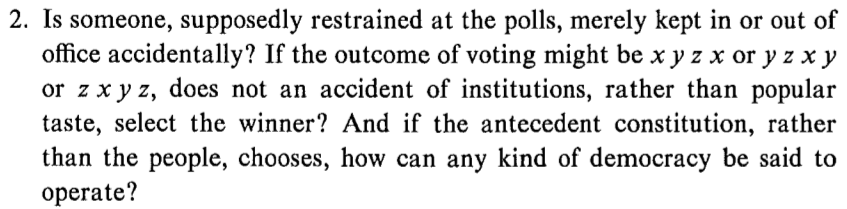
\includegraphics[width=\textwidth]{./pics/rk9.png} \\[0pt]

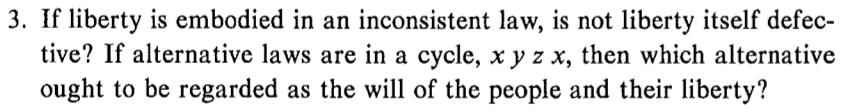
\includegraphics[width=\textwidth]{./pics/rk10.png} \\[0pt]

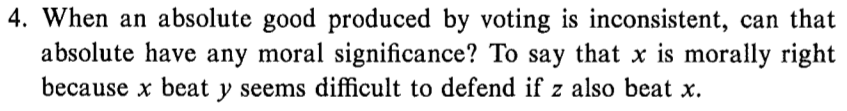
\includegraphics[width=\textwidth]{./pics/rk11.png}
\end{frame}
\begin{frame}[label={sec:org40a2db4}]{Las interrogantes liberales}
\begin{itemize}
\item ¿Puede una votación atar de manos al gobernante si el resultado de la votación es inconsistente? ¿Cómo opera la constricción si ni siquiera está claro cuál constricción impones?
\end{itemize}
\pause
\begin{itemize}
\item ¿No será que echas a un oficial, supuestamente constreñido por las urnas, por mera casualidad? Si el resultado puede ser \(x \; y\;  z \; x\), entonces es un accidente institucional, en vez del gusto popular, lo que selecciona al ganador. Y si decidiera una constitución accidental, y no el pueblo,  ¿cómo puedes afirmar que opera una democracia?
\end{itemize}
\end{frame}
\begin{frame}[label={sec:orgd2741ed}]{Las interrogantes rousseauvianas}
\begin{itemize}
\item Si la libertad se sustenta en una ley inconsistente, ¿no es defectuosa dicha libertad? Cuando hay ciclicidad de leyes alternativas, ¿cuál debería considerarse la voluntad general y su consecuente libertad?
\end{itemize}
\pause
\begin{itemize}
\item Cuando el bien absoluto que produce la votación es inconsistente, ¿tiene ese bien absoluto algún significado moral? Parece difícil decir que \(x\) es moralmente correcto porque vence a \(y\), cuando \(z\) también vence a \(x\)
\end{itemize}
\end{frame}
\end{document}
